\documentclass[a4paper,11pt]{article}
\usepackage[utf8]{inputenc}\usepackage[T1]{fontenc}
\usepackage[english]{babel}\usepackage{lmodern}\usepackage{microtype}
\usepackage{amsmath,amssymb}\usepackage{geometry}
\geometry{a4paper,left=2.2cm,right=2.2cm,top=2.0cm,bottom=2.0cm}
\usepackage{booktabs,array}\usepackage{xcolor}
\definecolor{bokug}{RGB}{0,135,60}\usepackage{tikz}
\usetikzlibrary{arrows.meta,calc}
\usepackage{fancyhdr}\pagestyle{fancy}
\renewcommand{\headrulewidth}{0.4pt}
\usepackage{enumitem}\setlength{\parindent}{0pt}\setlength{\parskip}{4pt}

\begin{document}
\fancyhead[L]{\small VU Mechanik – LAWI 100515 (PI)}\fancyhead[R]{\small SS 2026}\fancyfoot[C]{\thepage}
\begin{center}{\large\bfseries\color{bokug}University of Natural Resources and Life Sciences, Vienna (BOKU)}\\[2pt]{\large\bfseries VU Mechanik – LAWI 100515 (PI)}\\[4pt]Exam \textbf{Group A} \hfill Date: 26.06.2026\\[2pt]\rule{\linewidth}{0.4pt}\end{center}

\textbf{Given system}\par The planar system consists of bending beams and a truss connected by hinges.
\begin{center}
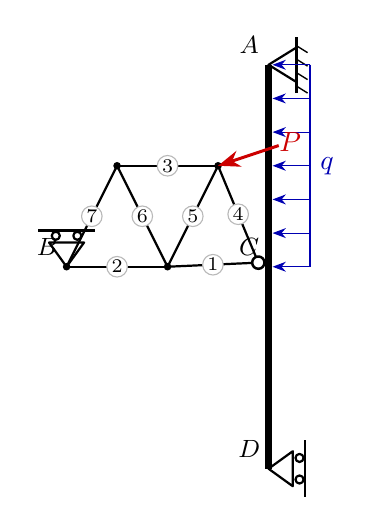
\begin{tikzpicture}[scale=0.855,>=Stealth,line join=round]
  \coordinate (P0) at (0.000,0.000);
  \coordinate (P1) at (0.000,-3.000);
  \coordinate (P2) at (0.000,-6.000);
  \coordinate (TO1) at (-1.500,-3.000);
  \coordinate (TO2) at (-3.000,-3.000);
  \coordinate (TU0) at (-0.750,-1.500);
  \coordinate (TU1) at (-2.250,-1.500);
  \coordinate (CPIN) at (-0.152,-2.939);
  \draw[thick] (CPIN) -- (TO1);
  \draw[thick] (TO1) -- (TO2);
  \draw[thick] (TU0) -- (TU1);
  \draw[thick] (CPIN) -- (TU0);
  \draw[thick] (TU0) -- (TO1);
  \draw[thick] (TO1) -- (TU1);
  \draw[thick] (TU1) -- (TO2);
  \draw[line width=2.2pt] (P0) -- (P1);
  \draw[line width=2.2pt] (P1) -- (P2);
  \fill (TO1) circle (1.6pt);
  \fill (TO2) circle (1.6pt);
  \fill (TU0) circle (1.6pt);
  \fill (TU1) circle (1.6pt);
  \draw[fill=white,line width=0.9pt] (CPIN) circle (2.6pt);
  \draw[thick] (0.000,0.000) -- (0.420,-0.260) -- (0.420,0.260) -- cycle;
  \draw[line width=1pt] (0.420,-0.420) -- (0.420,0.420);
  \draw[line width=0.5pt] (0.420,-0.320) -- (0.580,-0.420);
  \draw[line width=0.5pt] (0.420,-0.120) -- (0.580,-0.220);
  \draw[line width=0.5pt] (0.420,0.080) -- (0.580,-0.020);
  \draw[line width=0.5pt] (0.420,0.280) -- (0.580,0.180);
  \draw[thick] (0.000,-6.000) -- (0.360,-6.260) -- (0.360,-5.740) -- cycle;
  \draw[thick] (0.460,-6.160) circle (0.06) (0.460,-5.840) circle (0.06);
  \draw[line width=1pt] (0.540,-6.420) -- (0.540,-5.580);
  \draw[thick] (-3.000,-3.000) -- (-2.740,-2.640) -- (-3.260,-2.640) -- cycle;
  \draw[thick] (-2.840,-2.540) circle (0.06) (-3.160,-2.540) circle (0.06);
  \draw[line width=1pt] (-2.580,-2.460) -- (-3.420,-2.460);
  \node[circle,fill=white,draw=gray!55,inner sep=0.5pt,font=\scriptsize] at (-0.826,-2.970) {1};
  \node[circle,fill=white,draw=gray!55,inner sep=0.5pt,font=\scriptsize] at (-2.250,-3.000) {2};
  \node[circle,fill=white,draw=gray!55,inner sep=0.5pt,font=\scriptsize] at (-1.500,-1.500) {3};
  \node[circle,fill=white,draw=gray!55,inner sep=0.5pt,font=\scriptsize] at (-0.451,-2.220) {4};
  \node[circle,fill=white,draw=gray!55,inner sep=0.5pt,font=\scriptsize] at (-1.125,-2.250) {5};
  \node[circle,fill=white,draw=gray!55,inner sep=0.5pt,font=\scriptsize] at (-1.875,-2.250) {6};
  \node[circle,fill=white,draw=gray!55,inner sep=0.5pt,font=\scriptsize] at (-2.625,-2.250) {7};
  \draw[->,blue!70!black] (0.620,0.000) -- (0.060,0.000);
  \draw[->,blue!70!black] (0.620,-0.500) -- (0.060,-0.500);
  \draw[->,blue!70!black] (0.620,-1.000) -- (0.060,-1.000);
  \draw[->,blue!70!black] (0.620,-1.500) -- (0.060,-1.500);
  \draw[->,blue!70!black] (0.620,-2.000) -- (0.060,-2.000);
  \draw[->,blue!70!black] (0.620,-2.500) -- (0.060,-2.500);
  \draw[->,blue!70!black] (0.620,-3.000) -- (0.060,-3.000);
  \draw[blue!70!black,thick] (0.620,0.000) -- (0.620,-3.000);
  \node[blue!70!black] at (0.870,-1.500) {$q$};
  \draw[->,red!80!black,line width=1.1pt] (0.151,-1.200) -- (-0.750,-1.500);
  \node[red!80!black] at (0.322,-1.143) {$P$};
  \node[font=\small] at (0.000,0.000) [xshift=-7pt,yshift=7pt] {$A$};
  \node[font=\small] at (0.000,-3.000) [xshift=-7pt,yshift=7pt] {$C$};
  \node[font=\small] at (0.000,-6.000) [xshift=-7pt,yshift=7pt] {$D$};
  \node[font=\small] at (-3.000,-3.000) [xshift=-7pt,yshift=7pt] {$B$};
\end{tikzpicture}
\end{center}
\textbf{Given quantities:}\quad $a=3$\,m\quad $\ell=1,5$\,m\quad $h=1,5$\,m\quad $q=3$\,kN/m\quad $P=15$\,kN
\par\medskip
\textbf{Tasks}\par
\begin{enumerate}[label=\textbf{\arabic*.}]
  \item Determine the degree of static determinacy.
  \item Compute all support reactions and hinge forces.
  \item Determine all truss member forces (tension/compression).
  \item Draw the section forces $N$, $V$, $M$ of the bending beams.
\end{enumerate}
\end{document}